\section{Data Handling}\label{subsec:Scaling}
As previously mentioned, the data used in \ac{ML} is as, if not more, important than the model itself. 
As a consequence, there are several steps taken to ensure that the data is in a good state before 
we apply the \ac{ML} models to it. In this section I will discuss some of these aforementioned steps, both 
what they do and what each step hopes to achive.
\subsection{Feature Scaling}
The range of values for the different data features can vary immensely, and for most 
cost functions, this is a problem. For some features, a deviation on the magnitude 
of $10^3$ can be a good approximation, whereas for others it can be a vast 
overestimation. When a model is to define which direction it wants to tune, it is 
crucial that the errors across all features are weighted equally. Scaling aims to alleviate 
this issue by transforming all features to have a relatively equal range of values while
simultaneously preserving all information regarding each feature. Exactly how one chooses 
to scale the data heavily affects the performance of the model and is regarded as a hyperparameter 
of the model. 
\subsubsection{Standard Scaler}\label{subsubsec:StandardScalar}
In this analysis, I decided to use the highly popular scaling method, the \emph{standard scaler}. 
The standard scaler implemented in this study uses Scikit-learns's \texttt{StandardScaler}
\cite{StandardScaler}. The standard scaler function scales each feature individually by subtracting 
the mean and dividing by the standard deviation. In doing so the resulting scaled data has a mean 
of 0 and a standard deviation of 1. Mathematically the standard scaler, $\mathcal{S}$, transforms 
a data set, $X$, as 
\begin{align}
    \mathcal{S} \left(X\right) = \frac{X - \boldsymbol{\mu} _x}{\boldsymbol{\sigma}_x} ,
\end{align}
where $\boldsymbol{\mu} _x$ and $\boldsymbol{\sigma}_x$ are vectors with the elements being 
the mean and standard deviation for each feature, respectively.
\subsection{Principal Component Analysis}\label{subsec:PCA}
\acf{PCA} is a dimensionality reduction technique used in many analyses. The goal of
\ac{PCA} is to reduce the dimensions of a high-dimensional data set while at the same time conserving as 
much of the variance (or value spread) in the data as possible. The motivation behind dimensionality reduction 
is (mainly) rooted in two points. The first is noise reduction. Some features could not only be non-contributing 
during training, but could even introduce noise. The second reason is lack of convergence. In a large 
data set with many features and different classifications (in our case channels), a \ac{ML} could struggle
to identify the most important trends. By reducing the dimensionality in the data, the hope is that this 
would be easier. 
\\
In short, a \ac{PCA} finds the direction in the feature space along which the data has the largest 
variance (called principal components), using a linear combination of the original features, and projects the
data upon it, creating a new data set. The principal components are ordered such that the first captures the most variation,
the second captures the most variation orthogonal to the first and so on. Before applying the \ac{PCA}, it is essential to 
scale the data, to ensure a realistic representation of the variance in each feature.  We can summarize the algorithm of the 
\ac{PCA} in the following 6 steps:
\begin{enumerate}
    \item Center the data around 0 by subtracting the mean from each feature.
    \item Calculate the covariance matrix to find the covariance 
                             of each feature pair.
    \item Calculate the eigenvalue and eigenvectors of the covariance matrix.
    \item Order the eigenvector by size of the eigenvalues to define the directions 
                             in the feature space with the largest variance.
    \item Cast the data along these directions to form a new data set with 
                             the new features ranked from largest to lowest variance.
    \item Remove the features with the least variance according to some threshold
                            defined by the user.                      
\end{enumerate}
The threshold mentioned in the final point, is decided by the user, and defines how much of the variance from the original data 
set should be included. For example if the threshold is set to $70\%$, $X$ number of the last features will be removed such 
that at least $70\%$ of the variance is preserved.
\\
In figures \ref{fig:PCA1} and \ref{fig:PCA2} I have plotted the distribution of 10, 100 and 300 samples 
for the features with the most and second most variance (\ref{fig:PCA1}), and least and second least 
variance (\ref{fig:PCA2}) after applying \ac{PCA} to our data set. In this \ac{PCA} I am yet to remove features, 
so all four features are taken from a data set where all the variance is still conserved. Each color in the figures 
represent different categorize of collisions, i.e. $t\bar{t}$ or diboson. With this in 
mind, the different scales on the y- and x-axis ($10^0$ for figure \ref{fig:PCA1} and $10^{-8}$ for figure 
\ref{fig:PCA2}) exhibit how the \ac{PCA} creates new features where there is a vast difference in variance 
(and therefore value to the analysis), and justifies how one can remove features while preserving most of the variance. 
In figure \ref{fig:PCA2} we observe that all channels exhibit the same trends and are practically identical. 
In other words, these features would not contribute in training a model to distinguish the different channels. 
In comparison, figure \ref{fig:PCA1} displays large variance and individual trends among the different processes.
\begin{figure}
    \centering
    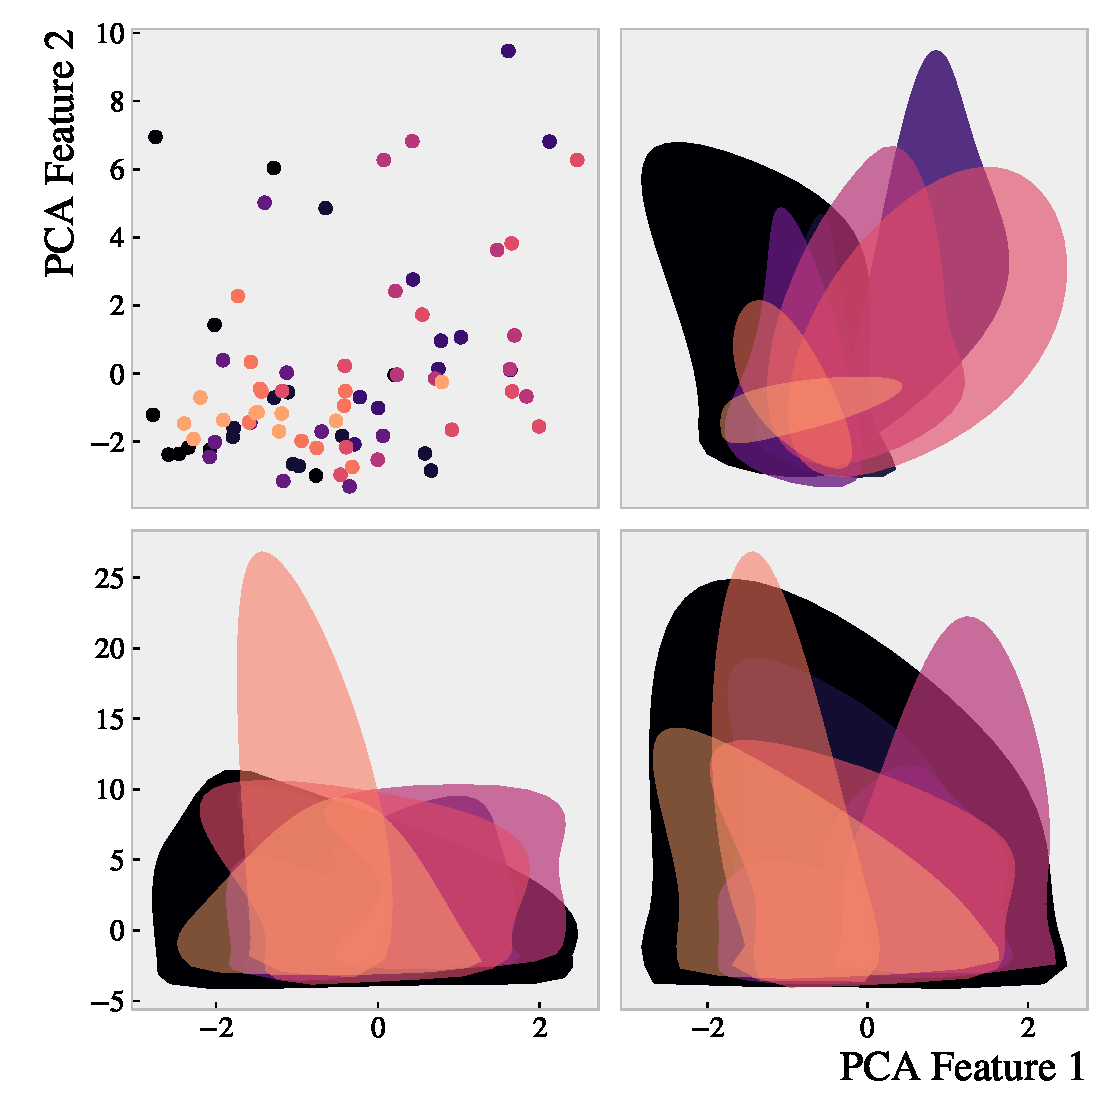
\includegraphics[width=0.6\textwidth]{Figures/MLResults/DataHandling/PCA/PCAPlotFirst.pdf}
    \caption[The value distribution of the two leading \acs{PCA}-features.]{The value distribution of 
    the two \ac{PCA}-features containing most variation for (left to right, up to down) 10, 10, 100 and 
    300 samples from each channel (visualized with different colors). Each sample filling the requirement with being less than one standard 
    deviation from the mean of both features, respectively.}
    \label{fig:PCA1}
\end{figure}
\begin{figure}
    \centering
    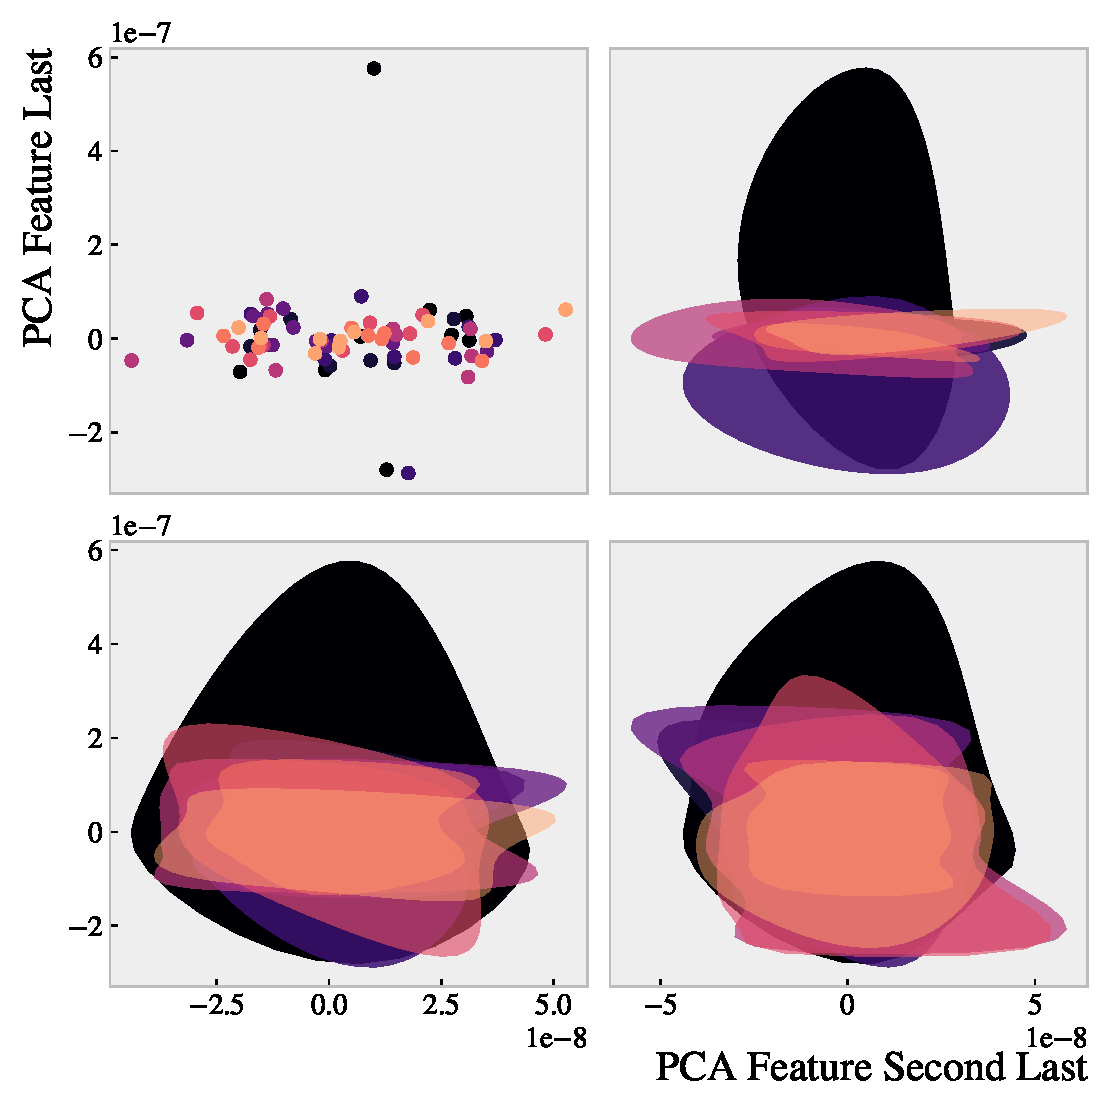
\includegraphics[width=0.6\textwidth]{Figures/MLResults/DataHandling/PCA/PCAPlotLast.pdf}
    \caption[The value distribution of the two last \acs{PCA}-features.]{The distribution of the two 
    \ac{PCA}-features containing the least amount of variation for (left to right, up to down) 10, 
    10, 100 and 300 samples from each channel (visualized with different colors). Each sample filling the 
    requirement with being less than one standard deviation from the mean of both features, respectively.}
    \label{fig:PCA2}
\end{figure}


